\ifx\PREAMBLE\undefined
\documentclass[fleqn]{article}
\usepackage{geometry}
\usepackage[format = hang, font = bf]{caption}
\usepackage{subcaption}
% The following is needed in order to make the code compatible
% with both latex/dvips and pdflatex. Added for using UML generated by MetaUML.
\ifx\pdftexversion\undefined
\usepackage[dvips]{graphicx}
\else
\usepackage[pdftex]{graphicx}
\DeclareGraphicsRule{*}{mps}{*}{}
\fi
\usepackage{array}
\newcolumntype{C}[1]{>{\centering\let\newline\\\arraybackslash}b{#1}}
\newcommand{\parcell}[2][l]{\begin{tabular}{@{}#1@{}}#2\end{tabular}}
\usepackage{pdflscape}
\usepackage{multirow}
\usepackage{graphicx}
\usepackage{floatrow}
\floatsetup[table]{capposition=top}
\usepackage{bigstrut}
\usepackage{supertabular}
\usepackage{booktabs}
\usepackage{amsmath}
\usepackage{listings}
\usepackage{multicol}
\usepackage{xcolor}
\usepackage{mathrsfs}%mathcal
\usepackage{amsfonts}%allowing \mathbb{R}
\usepackage{amssymb}
\usepackage{alltt}
\usepackage{xspace}
\usepackage{color}
\usepackage{wrapfig}%text around figure
\usepackage{lipsum}
\usepackage{tikz}
\usetikzlibrary{shapes,positioning}
\usepackage{url}
\def\UrlBreaks{\do\A\do\B\do\C\do\D\do\E\do\F\do\G\do\H\do\I\do\J\do\K\do\L\do\M\do\N\do\O\do\P\do\Q\do\R\do\S\do\T\do\U\do\V\do\W\do\X\do\Y\do\Z\do\[\do\\\do\]\do\^\do\_\do\`\do\a\do\b\do\c\do\d\do\e\do\f\do\g\do\h\do\i\do\j\do\k\do\l\do\m\do\n\do\o\do\p\do\q\do\r\do\s\do\t\do\u\do\v\do\w\do\x\do\y\do\z\do\0\do\1\do\2\do\3\do\4\do\5\do\6\do\7\do\8\do\9\do\.\do\@\do\\\do\/\do\!\do\_\do\|\do\;\do\>\do\]\do\)\do\,\do\?\do\'\do+\do\=\do\#\do\-}
\usepackage{xr}%allow cross-file references
\usepackage[breaklinks = true]{hyperref}
\lstset{
language = C, 
showspaces = false,
breaklines = true, 
tabsize = 2, 
extendedchars = false, 
basicstyle = {\ttfamily \footnotesize}, 
showstringspaces=false,
keywordstyle=\color{blue!70}, 
commentstyle=\color{gray},
rulesepcolor=\color{red!20!green!20!blue!20}, 
numberstyle=\color[RGB]{0,192,192},
stringstyle=\color{red},
escapeinside={ )},
moredelim=[is][\underbar]{(**}{**)},
mathescape
}
\mathchardef\myhyphen="2D
\begin{document}
\fi
\newpage
\section{Memory Hierarchy}
\subsection{Storage Technologies}
\begin{description}
\item[RAM]Random Access Memory. SRAM is faster (10$\times$) but more expensive (1000$\times$) than DRAM.
\item[SRAM]Static Random Access Memory. Each bit is stored in a bistable memory cell. It can stay indefinitely in one of the two voltage configurations. Insensitive to disturbance.
\item[DRAM]Dynamic Random Access Memory. Each bit is stored as charge on a capacitor. Sensitive to disturbance. 
\begin{figure}[ht]
\centering
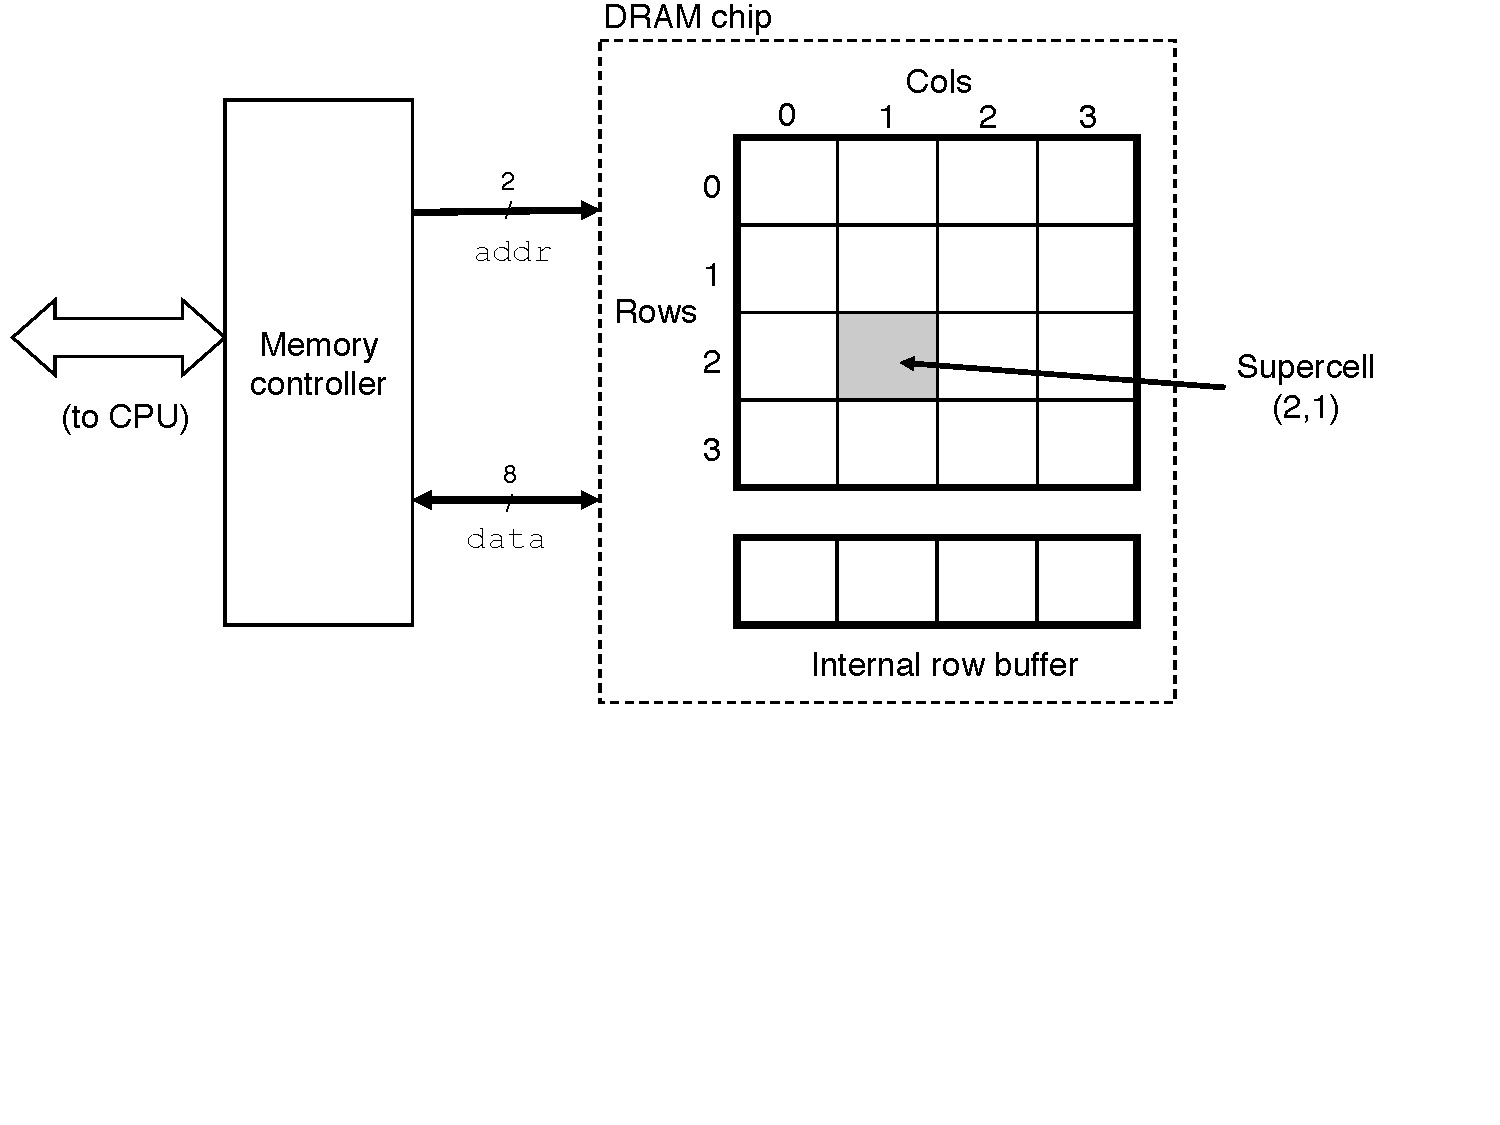
\includegraphics[width=0.6\textwidth]{dram.pdf}
\caption{A 128 bit (16$\times$8) DRAM chip}
\end{figure}
\begin{description}
	\item[FPM DRAM]Fast Page Mode DRAM.
	\item[EDO DRAM]Extended Data Out DRAM.
	\item[SDRAM]Synchronous DRAM.
	\item[DDR SDRAM]Double Data-Rate SDRAM.
	\item[VRAM]Video RAM.
\end{description}
\item[RAS/CAS]Row/Column Access Strobe. Row/Column address sent from the memory controller to the DRAM chip.
\item[ROM]Read-Only Memory. (Nonvolatile Memory).
\item[PROM]Programmable ROM. Programmable only once.
\item[EPROM]Erasable PROM. Programmable \~{}1000 times.
\item[EEPROM]Electrically Erasable PROM. Programmable \~{}$10^5$ times. \textbf{Flash memory} is based on EEPROM. \textbf{SSD}(Solid State Disk) is based on flash memory.
\item[Firmware]Programs stored in ROM.
\item[Bus]Data flows between CPU and DRAM main memory through the buses. Each data transfer is called a \textbf{bus transaction}, either \textbf{read transaction} or \textbf{write transaction}.
\item[Disk]Platter, surface, spindle, cylinder, track, sector, gap. Rotation rate, RPM(Revolution Per Minute).
\begin{figure}[ht]
\ffigbox[\textwidth]{}{{
\begin{subfloatrow}[2]
\ffigbox[0.5\textwidth]{\caption{Single platter}}{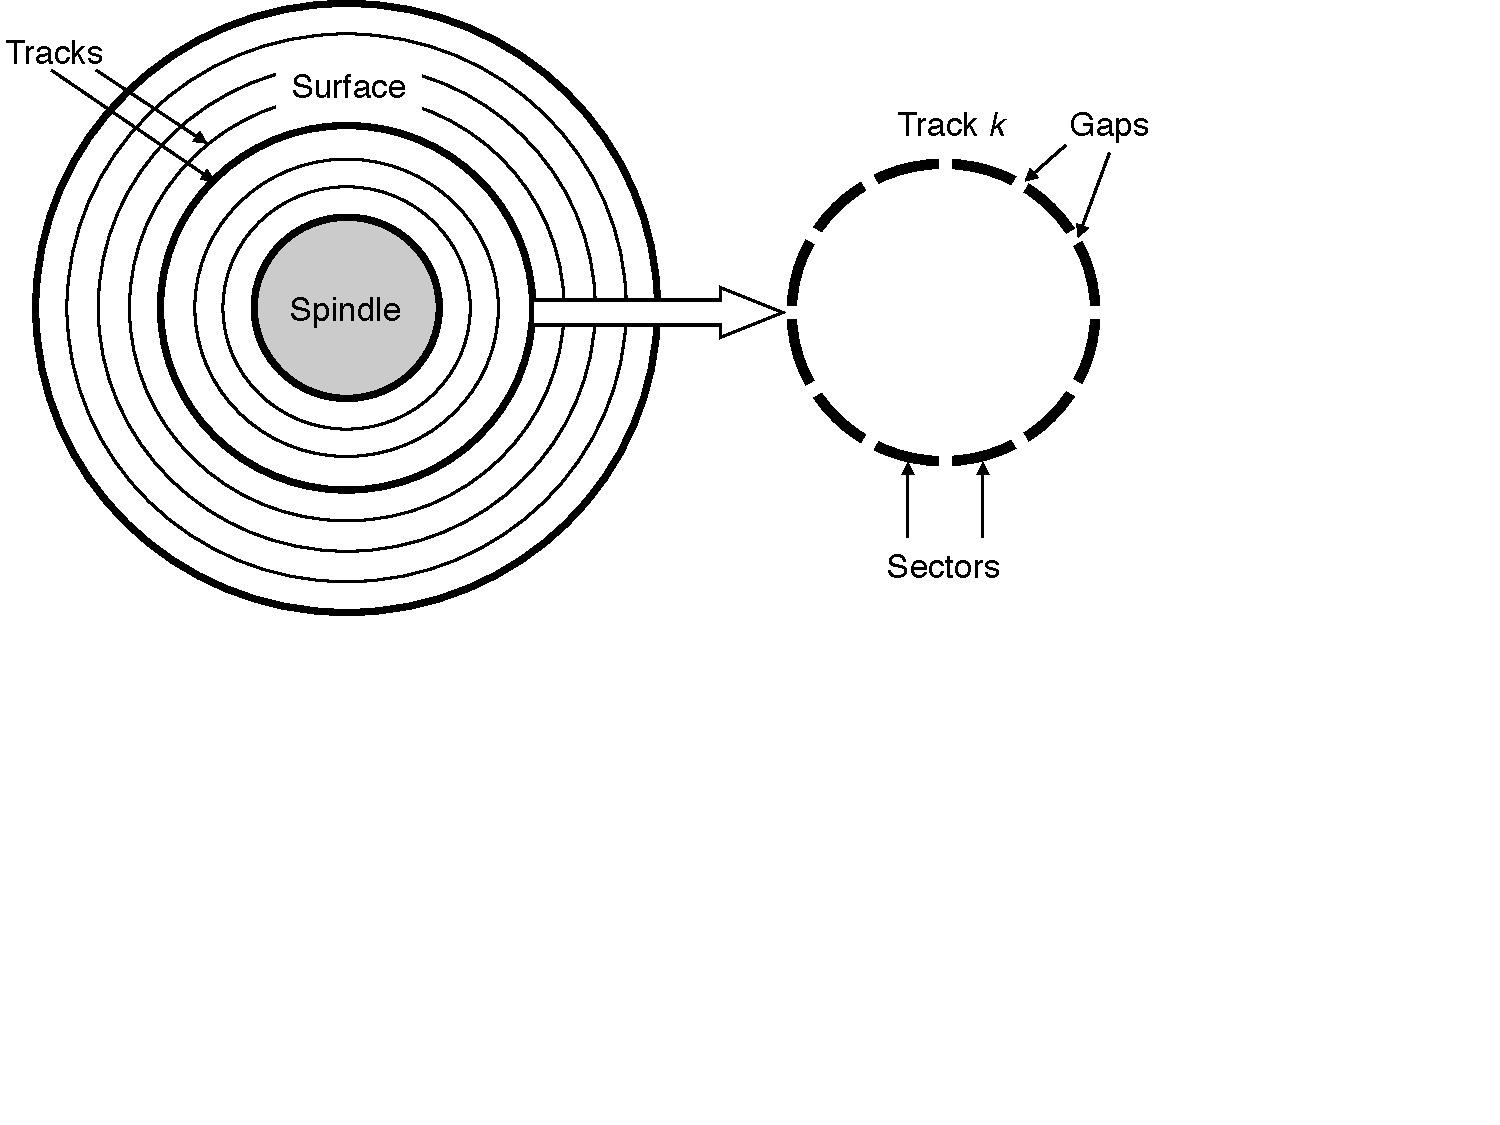
\includegraphics[width=0.5\textwidth]{surface.pdf}}
\ffigbox[0.5\textwidth]{\caption{Multiple platters}}{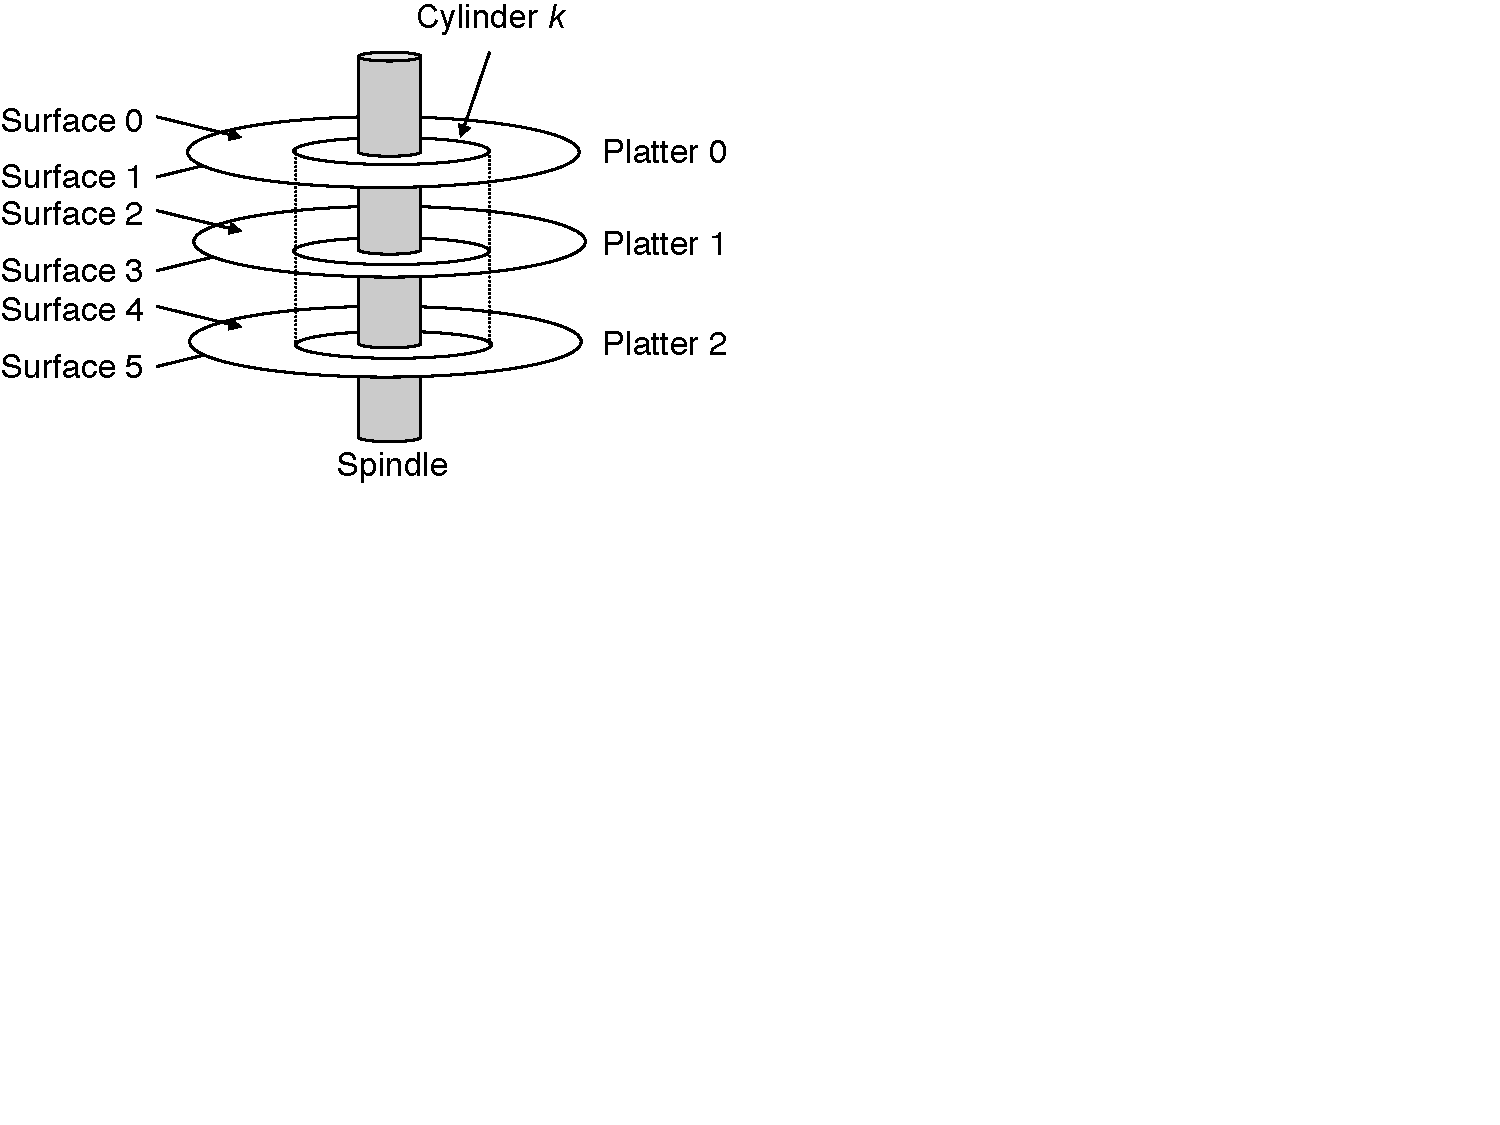
\includegraphics[width=0.5\textwidth]{cylinder.pdf}}
\end{subfloatrow}}
\caption{Disk geometry}}
\end{figure}
\[Capacity=\frac{Bytes}{Sector}\times\frac{Sectors}{Track}\times\frac{Tracks}{Surface}\times\frac{Surfaces}{Platter}\times\frac{Platters}{Disk}\]

Access time:
\begin{itemize}
\item Seek time: $T_{\text{avg seek}}=3\sim 9\:ms$.
\item Rotational latency: $T_{\text{avg rotation}}=\frac{1}{2}\times\frac{1}{RPM}\times\frac{60s}{1min}\sim T_{\text{avg seek}}$
\item Transfer time: $T_{\text{avg transfer}}=\frac{1}{RPM}\times\frac{1}{Sectors/Track}\frac{60s}{1min}\ll T_{\text{avg seek}}$.
\end{itemize}

Disk controller maintains the mapping between logical blocks and physical disk sectors. 

\item[I/O Bus] Unrelated to CPU. Intel: PCI(Peripheral Component Interconnect) bus. Connects to:
\begin{itemize}
	\item USB(Universal Serial Bus) controller: connects to USB devices.
	\item Graphics card/adapter.
	\item Host bus adapter: connects to one or more disk drives.
\end{itemize}
\begin{figure}[ht]
\centering
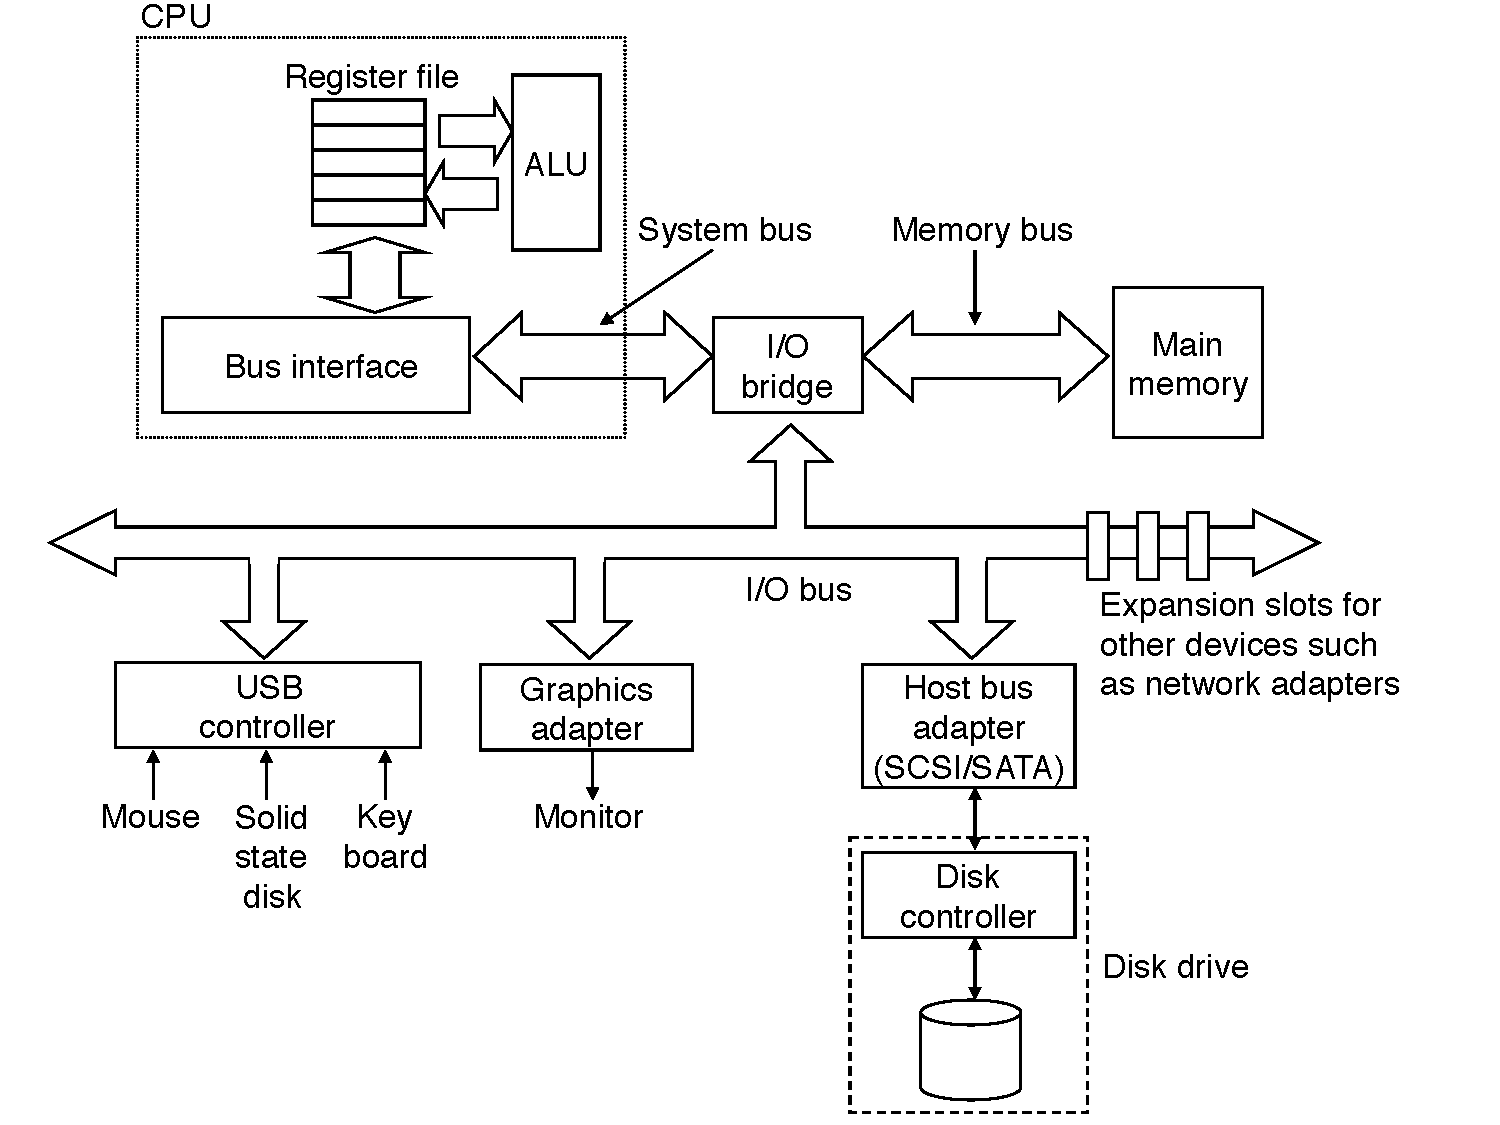
\includegraphics[width=0.6\textwidth]{iobus.pdf}
\caption{System bus, memory bus, IO bus}
\end{figure}
\item[Memory mapped I/O]CPU uses memory-mapped I/O to send instructions to I/O devices via I/O ports, i.e. a series of special addresses in the memory space.
\item[DMA]Direct Memory Access. I/O devices carry out read/write transactions without interference of CPU. 
\end{description}
\subsection{Locality \& memory hierarchy}
\begin{itemize}
	\item Temporal locality \& spacial locality
	\item Stride-k reference pattern: stride-1 reference pattern has the best spacial locality.
	\item Memory hierarchy \& typical visit time: Register (0) - L1 SRAM cache (4) - L2 SRAM cache (10) - L3 SRAM cache (50) - Main DRAM memory (200) - Hard disk (10000000) 
\end{itemize}
\subsection{Cache memories}
\begin{figure}[ht]
\centering
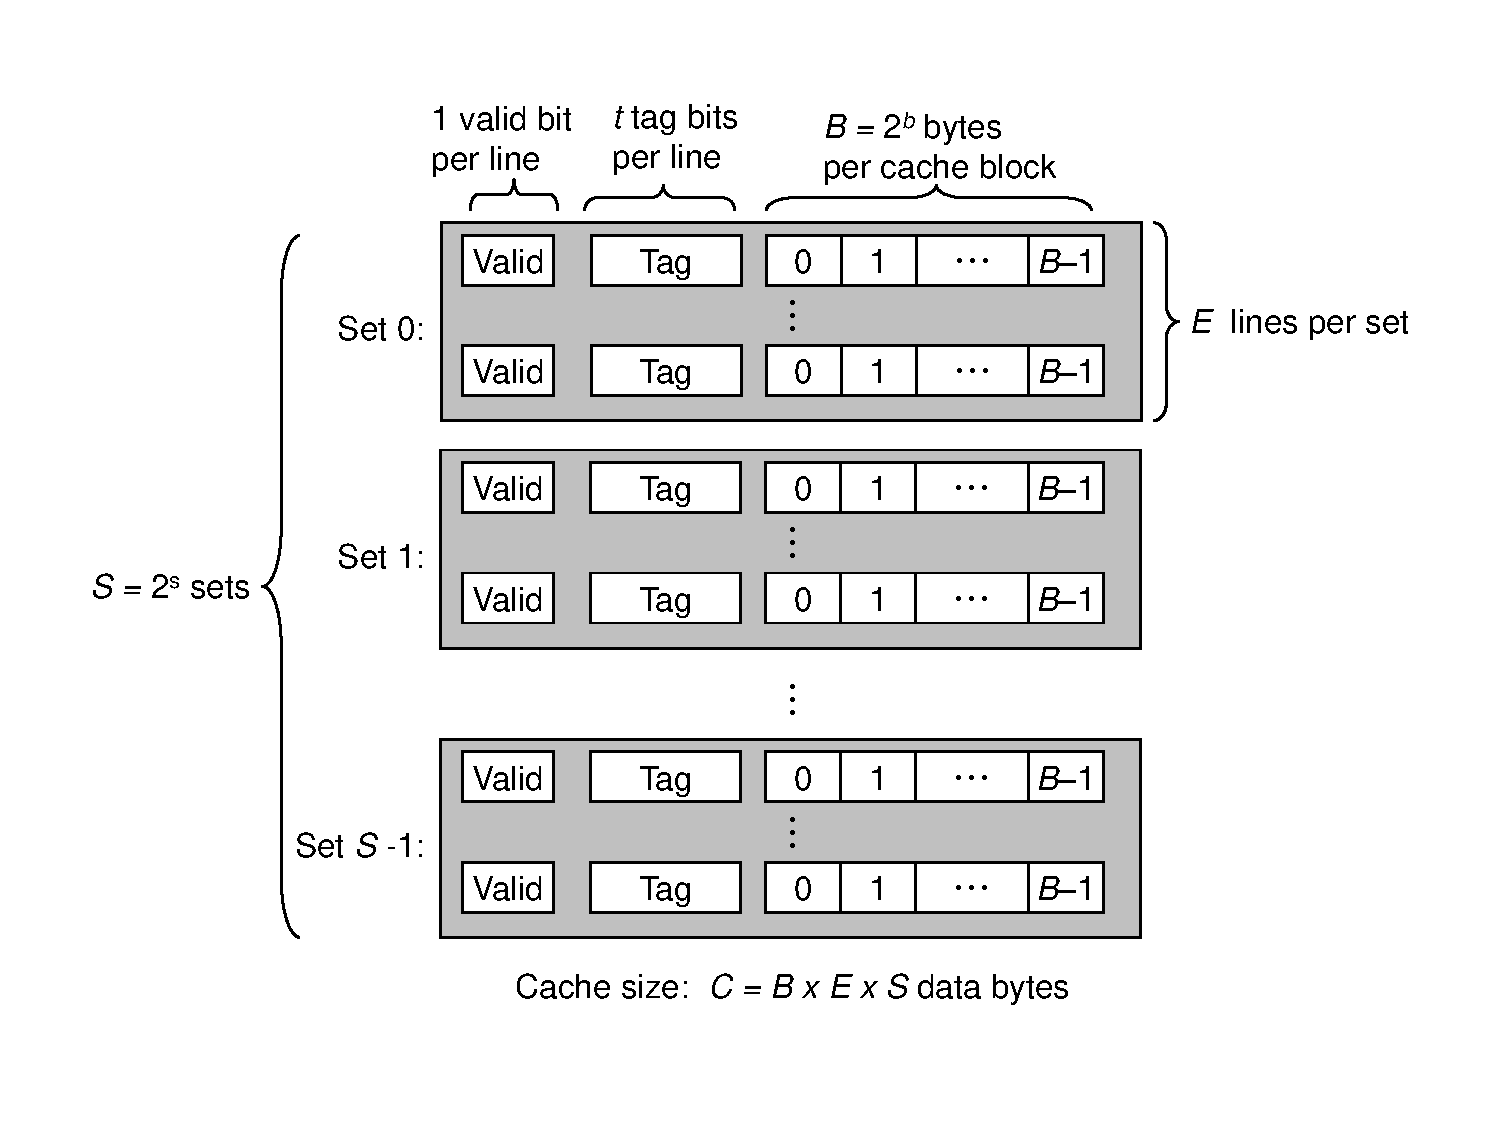
\includegraphics[trim=30 50 30 50, clip, width=0.75\textwidth]{cacheorg.pdf}
\caption{Organization of cache memory(S,E,B,m)}
\end{figure}
\begin{itemize}
\item m-bit address: t-bit tags + s-bit set index + b-bit block offset.
\item Direct-mapped cache: $E = 1$. E-way set associative cache: $1<E<C/B$. Full associative cache: $S=1$.
\item 3 steps: set selection; line matching; word extraction. In case of cache miss: line replacement.
\item Cache thrash: cache keeps loading \& evicting the same blocks.
\item Handle write: write-through (directly write to lower layer) v.s. write-back (put off write until line gets replaced).
\item Handle write cache miss: write-allocate (load from lower layer then update) v.s. not-write-allocate (directly write to lower layer).
\item Usually: write-through + not-write-allocate; write-back + write-allocate.
\item Write cache-friendly code: improve cache hit rate. For example, to write code for matrix multiplication $C=A\times B$, instead of straightforwardly writing:\\
\begin{tabular}{m{180pt}m{180pt}}
\begin{lstlisting}
//ijk
for(i = 0; i < n; ++i)
	for(j = 0; j < n; ++j) {
		sum = 0.0;
		for(k = 0; k < n; ++k)
			sum += A[i][k] * B[k][j];
		C[i][j] = sum;
	}
\end{lstlisting}
&
\begin{lstlisting}
//kji
for(k = 0; k < n; ++k)
	for(j = 0; j < n; ++j) {
		r = B[k][j];
		for(i = 0; i < n; ++i)
			C[i][j] += A[i][k] * r;
	}

\end{lstlisting}\\
\end{tabular}\\
we should write:
\begin{lstlisting}
//ikj
for(i = 0; i < n; ++i)
	for(k = 0; k < n; ++k) {
		r = A[i][k];
		for(j = 0; j < n; ++j)
			C[i][j] += r * B[k][j];
	}
\end{lstlisting}
\begin{table}[ht]
\caption{Analysis of different inner loops}
\centering
\begin{tabular}{c|c|c|c|c|c|c}\toprule
version & load & store & A miss & B miss & C miss & total miss\\\midrule
ijk \& jik & 2(AB) & 0 		& 0.25 & 1.00 & 0.00 & 1.25\\\midrule
kji \& jki & 2(AC) & 1(C) & 1.00 & 0.00 & 1.00 & 2.00\\\midrule
ikj \& kij & 2(AC) & 1(C) & 0.00 & 0.25 & 0.25 & 0.50\\\bottomrule
\end{tabular}
\end{table}

\end{itemize}
\ifx\PREAMBLE\undefined
\end{document}
\fi